% \documentclass[rnd]{mas_proposal}
\documentclass[thesis]{mas_proposal}

\usepackage[utf8]{inputenc}
\usepackage{amsmath}
\usepackage{amsfonts}
\usepackage{amssymb}
\usepackage{graphicx}

\title{Real-time Learning from Demonstration under Graph-World representation}
\author{Natalia Leonila Quiroga Perez}
\supervisors{Prof. Dr. Paul G. Plöger\\
	Dr. Alex Mitrevski \\}
\date{July 2023}

% \thirdpartylogo{path/to/your/image}

\begin{document}

\maketitle

\pagestyle{plain}

\section{Introduction}

\subsection{Topic of This  Project / Learning from Demonstration }\
\begin{itemize}
    \item Provide reasonably detailed description of what you intent to do in your Master Thesis.
    \item You may also discuss the challenges that you have to address.
    \item Reflect on the profile of the reader and PLEAAAASE, tell a story here and refrain from bombarding the readers with details which they may not be able to appreciate.
\end{itemize}

    Due to the growing acceptance of the use of robots in collaboration with humans in the same environment, Human-Robot Interaction (HRI) is being studied as a successfully emerging area. According to \cite{Sheridan2016}, there are four areas of application of HRI; namely, (i) human resources as supervisors in different areas where the tasks are repetitive but robots are still not independent (ii) robots that work in hazardous environments where humans do not have access, and whose movements are usually controlled remotely by an expert, (iii) autonomous robots, such as self-driven cars with humans as passengers, those navigate and plan by sensing their environment, and finally, (iv) robots in a social environment where they interact directly with people, teaching, entertaining, helping children and the elderly.
    
    Specifically, focusing on human-robot social interaction applications, robots used in therapy with children with Autism Spectrum Disorder (ASD) had a positive impact on the patients, as the children had certain preferences for the robot as a therapist instead of an adult; according to \cite{Prabha2019}, this is because children with this condition perceive the world differently and robots attract their attention.
    
    In order to encourage patients with autism to learn movements and body language during therapy, the typical procedure is human-human encounters; namely, a selection of imitation games are performed as described in \cite{Dautenhahn2004}, where the authors are aware that robots have limited movements, and this method would be difficult to use in a long term therapy, unless the robots increase their behavioural repertoire.
    
    Various procedures can be performed in order to increase the action libraries for the robots. From the naive approach of encoding each and every action, to the more sophisticated approach of using methods to collect demonstrations from humans include different types of motion capture such as kinesthetic guidance \cite{Kronander2013}, joystick control \cite{Jiang2013} and kinect camera\cite{Assad2020}. Collecting a large number of these demonstrations from non-experts to perform a motion learning procedure is not feasible and tedious for the demonstrator \cite{Chen2022}.
    
    During the study of robots in therapy for ASD, most of the time the main focus are the patients and how the robot affects their reaction, but the therapist also have a reaction to the involvement of robots. In the study by \cite{Kulikovskiy2021}, the therapists are the main focus and their preferences are explored, if they do not feel comfortable with the inclusion of new technology and they do not understand how to use it, it may be the case that they go back to traditional methods.
    
    Therapists, as part of the end-user group, should be able to operate the robots with little training and effort. During the experiments performed by \cite{Kulikovskiy2021}, with real therapists and the robot Pepper, the main observations were: (i) therapists prefer to teleoperate the robot with Virtual Reality (VR) than to manipulate the robot with a kinesthetic interface; (ii) the use of VR provides a treatment integrity of 83.7\%, which is comparably higher than the 52.9\% of the kinesthetic interface; (iii) therapists found it easier to adapt the therapy to the children's needs with the use of VR; and finally (iv) the workload of task preparation was higher with VR than with kinesthetic interface. 
       
    For instance, the aim is to simplify this process for the demonstrator by making it more user-friendly and faster. The human ability to learn by imitation, and social mirroring \cite{Byrne2005}, inspired Learning from Demonstration (LfD), which has now become an area of extensive research.
    
    In LfD it is necessary to collect examples of optimal sequences of actions or trajectories in order to reproduce similar behaviours \cite{Piot2017}. This can be achieved in two ways; on one hand, Imitation Learning (IL) is a type of supervised learning that consists of learning the mapping between states and actions \cite{Dinyari2020}. On the other hand, Inverse Reinforcement Learning (IRL) has no knowledge of the reward function and tries to learn from the expert's demonstrations \cite{Reddy2019}.
    
    The aim of this project is to create a framework that facilitates the process of learning upper limb body movements to extend the action repertoire of robots by capturing skeletal data from non-expert users using an external camera. Subsequently, this library will be stored in order to use the movements in therapy with ASD patients.
    
    The functionality of the framework is divided into two phases, one of which is carried out only once before the non-expert starts the demonstrations; namely, the robot has to carry out a discretization of the environment by performing a space exploration within the limits of the actuators in order to map and recognise the environment and possible obstacles present in its workspace, including its own body structure. The result of this exploration is a set of $n$ graphs, where $n$ is the number of joints of the robot. Each joint graph $i$ has a dependency on the graph $i-1$ of the previous joint. The vertices or nodes represent a reachable point for joint $i$ in the Cartesian space and it stores the position $(x, y, z)$, the joint angles of all previous joints $(1,2,..,i)$ as $(\theta_1, \theta_2,..,\theta_i)$, a state of free or occupied $(0, 1)$, and a list of $k$ joints that can reach the same spatial position in some configuration, it means that this point exists in at least one other graph. 	
 	The edges of all graphs are the Euclidean distance $(d)$ between two nodes, the value of $d$ is constant and determines the quality of the discretisation; namely, the smaller the value of $d$, the higher the quality of the graphs, which means the quality of the movements, the search time and the memory storage also increase; if the value of $d$ is larger, the memory storage and the search time are smaller, but the quality of the path is compromised. Therefore, $d$ has to be carefully tuned to a value that does not compromise either the movements or the time and memory costs.
 	
	The second phase of the framework assumes that the space is partially known to the robot, due to the fact that not all points of the Cartesian space may be explored or there may be more than one robot configuration to reach that point, but enough points have been collected to avoid self-collisions and to detect the static obstacles.  The demonstrations can then be carried out. The skeleton-based data stores the position of the human embodiment. Considering the skeleton upper body part, the joint called "collar" is placed in the center of the body near the chest, this is for the human the base frame $B^H = (0, 0, 0)$, continuously, we can calculate the Spherical coordinates for all the human joints following the equations \ref{eq:radial_distance}, \ref{eq:polar_angle} and \ref{eq:azimuthal_angle}.
	
	\begin{equation}
		 r = \sqrt{x^2 + y^2 + z^2}
	\label{eq:radial_distance}
	\end{equation}
	\begin{equation}
		\theta = \arctan \frac{y}{x}
	\label{eq:polar_angle}
	\end{equation}
	\begin{equation}
		\phi = \arctan \frac{\sqrt{x^2 + y^2}}{z}
	\label{eq:azimuthal_angle}
	\end{equation}

	The transformation gives the polar angle and the azimuthal angle which are the direction of all links. These are then used to calculate the Cartesian coordinates of the robot on its own embodiment following the equations \ref{eq:x_cartesian}, \ref{eq:y_cartesian} and \ref{eq:z_cartesian}. 
	
	\begin{equation}
		x = r \sin \phi \cos \theta
		\label{eq:x_cartesian}
	\end{equation}
	\begin{equation}
		y = r \sin \phi \sin \theta
		\label{eq:y_cartesian}
	\end{equation}
	\begin{equation}
		z = r \cos \phi
		\label{eq:z_cartesian}
	\end{equation}
	Once the desired pose of the robot is found, i.e. the coordinates $(x,y,z)$ of all the joints in Cartesian space, it is possible to search for these coordinates for each joint on its corresponding graph. This would lead to a specific angular configuration for all captured frames. Given the characteristics of the RealSense Depth Camera used, namely its frame rate for RGB of up to 30 fps \cite{realsense_manual}. Therefore, not all frames can be reproduced in real time and the trajectory is compromised, e.g. the positions should be selected wisely during the learning process under certain constraints. After learning, the path found can be reproduced in the robot.

\subsection{Constraints}
	In this section, the constraints necessary to perform path planning within the discretised representation of the world are introduced.
	\begin{itemize}
		\item IsInside($p$, $j$): The Cartesian points $p$ found for all joints must be inside the workspace of the respective joint $j$. The robot's workspace is not the same workspace for each joint.
		\item IsNode($p$, $g_j$): The Cartesian point $p$ found for all joints is already a node in the graph $g_j$ if the corresponding joint is $j$. If it is not a node and it is inside the workspace, then find the nearest node. If the distance between the candidate node $N_{candidate}$ and the closest node $N_{closest}$ is smaller than the value of the fixed edge $d$ then $N_{closest}$ is added to the path and no new node is created.
		\item CreateNode($p$, $g_j$, $\Theta$, $occupied$): If the distance between $N_{candidate}$ and the closest node $N_{closest}$ is greater than $d$, then the candidate is added to the graph $g_j$ with the corresponding angular configuration of the angles to reach that position. The state "occupied" is initialised with 1 or TRUE. This new node depends on the previous node where the joint was. For instance, there is a direct connection between these two nodes and the node $N_{candidate}$ is added also to the path.
	\end{itemize} 
\subsection{Real-Time Path Planning}
	This section defines the necessary terms to perform real-time path planning. Namely, it describes search, learning and execution. 
	\subsubsection{Search}
		The search consists of finding a path on the existing graphs that best represents the trajectory that the user is performing. This must be done while the demonstration is being recorded. The initial position of the paths is always the robot's home position, which is a known configuration of nodes. On the other hand, the target position is unknown throughout the demonstration, the goal is represented by a configuration of nodes.	
	\subsubsection{Learning}
		The system must be able to learn after each demonstration. Lifelong learning is applied in a way that the graphs should extend their stored information as wisely as the trajectory libraries increase.
	\subsubsection{Execution}
		The execution consists of smoothing the captured path to reproduce an optimised set of nodes that are representative of the movement. 
\subsection{Relevance of This Master Thesis}
\begin{itemize}
    \item Who will benefit from the results of this project?
    \item What are the benefits? Quantify the benefits with concrete numbers.
    \item 
    \item 
    \item 
 \end{itemize}

\section{Related Work}

	\subsection{Survey of Related Work}
	\begin{itemize}
		\item What have other people done to solve the problem?
		\item You should reference and briefly discuss at least the ``top twelve'' related works
	\end{itemize}
	
	\subsubsection{Autism Therapy}
		Patients with autism have problems with communication in general, as well as repetitive behaviours and restricted interests. During diagnosis, according to \cite{Brentani2013}, it is possible to identify the syndrome by noticing a lack of social interaction and affection with others, as well as repetitive body postures and lack of eye contact.  Depending on the level of autism, the treatment and synthoms may vary but in general the main focus is to increase their level of communication, this can be done by understanding non-verbally other people; namely understanding the tone of their voice, body posture, facial expressions and hand motions. As they tend to copy repetitive gestures \cite{Dautenhahn2004}, the therapy usually include repetition of movements that the patient has perform. These restricted and repetitive behaviours (RRBs) are implemented in an early age and tend to reduce as time goes by and the patients' cognitive ability increases \cite{Leekam2011}. ASD experts propose that the earlier the therapeutic intervention, the better the development of a normal adult life. Many treatments involve external assistance such as pets, computers, virtual reality, and robots, some of which have positive results compared to others, but also therapy may vary from patient to patient \cite{Scassellati2012}.
		
	\subsubsection{Learning from Demonstration}
		Robots are those designed to interact with humans. In most cases these robots have a humanoid shape or appearance, but the degrees of freedom (DOF) vary between them, some examples are Kaspar with 17 DOF\cite{Kaspar2023}, QTrobot with 12 DOF \cite{qtrobot_safety_manual}, Nao with 25 DOF \cite{softbankrobotics}, Pepper with 20 DOF \cite{softbankrobotics} and Zeno with 12 DOF \cite{Papakostas2021}. Given the large number of DOF they represent, programming them became a difficult task even for experts. Nevertheless, this difficulty leads to methods of autonomous learning; namely, learning by demonstration. This learning process tends to be natural and intuitive for the demonstrators, i.e. they should not be given long sets of technical instructions; demonstrations are safer for the robot than using a trial-and-error learning process, which can damage the robot and takes longer for each new learned movement \cite{Bandera2012}. Ideally, direct mapping can be performed, but the number of DOF become a problem, and direct mapping is not recommended in uncontrolled environments due to the possibility of collision with external agents or objects \cite{Bentivegna2004}.
	
		However, considering that human and robot bodies have similar general characteristics, a one-to-one mapping is possible in some cases. Nevertheless, it is important to contemplate the following strategies considering the DOF; one-to-many, many-to-one or many-to-many mapping \cite{Alissandrakis2007}. In all cases, it is necessary to have a clear understanding of what is the expected result of the mimicking and which strategy to follow; for example, the movement has to maintain certain angular configuration to avoid obstacles or the position of the end effector has to be maintained \cite{Bandera2010, Shin2001}.
		
		The imitation learning task is divided into two important parts: (i) the observation process, which involves data collection, and (ii) the imitation process, where the imitator can follow three strategies to imitate: the end-point level, where only the position and orientation of the end effector matter, the trajectory level, where velocity matters, and the path level, where spatial properties matter more than velocity \cite{Alissandrakis2002}.
		
		For the observation process, various approaches use external hardware such as touch sensors, cameras and external devices to accurately identify the target pose \cite{Hua2021}. Previous work such as \cite{Itauma2012, Liu2015} uses a Kinect sensor to track the human skeleton model to estimate the human pose, but the experiments are affected by sensor quality, light exposure and processing speed. Other approaches use a mobile phone to create the path for the robot, the device is moved as required and the robot follows the path. These experiments require a set of training data, and the results depend on the number of attempts made by the user; in particular, if there is one failed sample, the failure needs to be compensated for by many more correct samples \cite{Mandlekar2018}. In order to analyse the skeleton data, it is necessary to formalise a mathematical expression that optimises an imitation metric \cite{Billard2004}; this procedure can be done with the help of a geometric model such as Denavit-Hartenberg (DH) \cite{Fadli2018}. \cite{Assad2020} \cite{VanPerre2015}, which describes the relationship between successive joints and is used to place each of them in a given coordinate frame using a Homogeneous Transformation (HT) to calculate the relative position of each joint. Finally, some authors replace visual inputs with other types of data, such as markers, but these are often invasive and must be used in controlled environments to avoid disturbance; in particular, one of the common failures of this approach is its poor adaptability to natural environments \cite{Mohammad2009, Dillmann2004}.
		
		Of course, IL has disadvantages. Given that human movements are intended to be learned, it is challenging to apply this procedure to a non-humanoid robot. The ideal scenario would be to have a robot with a human-like shape and the same number of DOF moving in a similar way, but this is rarely the case \cite{Ravichandar2020}. Most applications using IL only consider the upper body, as shown in \cite{VanPerre2015}, due to the complex control system that requires the legs to move. Another important factor to mention is that these works do not take into account the speed of movement of the robot joints, which can cause damage to the structure. 
		
	\subsubsection{LfD in Therapy}
		In the context of therapy and rehabilitation, especially in the treatment of autism, showing a patient movements to imitate is a very efficient technique to learn movements or to associate them with an activity; in addition, this can also help to the patients to relate places with everyday movements. Therefore, they can perform independently certain activities, such as brushing their teeth, cleaning themselves and other basic needs. According to \cite{Cabibihan2013}, 6\% of robots that they mention are adaptable to the user's needs. The adaptability of the robot is important, not just because the environment where the interaction occurs, but more important, to modify and customize progressively the complexity of the therapy \cite{Dickstein2018}. The behavioural repertoire of the robot is usually limited. Programming new postures or sets of movements is a complicated task that requires a lot of time, effort and knowledge in the field of robot programming and control.
		
		Imitation learning in robotics has many advantages for the end user. As there is no need to create programmes for each task or action, no technical knowledge is required, complex postures can be achieved and the learning effort can be reduced. More specifically, in this application we focus directly on the needs of the therapist \cite{Ravichandar2020, Kulikovskiy2021} and indirectly on the needs of the patient. 	

	\subsubsection{One-shot Learning}

		One-shot learning attempts to learn the action after each demonstration without prior training \cite{Yan2010}; for example, this type of technique can overcome the problem of insufficient samples while still producing an expected result. A skeleton-based method for dynamic hand gesture recognition using a reinforcement learning network (GREN) based on one-shot learning is proposed in \cite{Chunyong2020}, where only a small subset of gestures from a dataset was taken as training samples; in an evaluation experiment, given 14 classes, the final accuracy achieved was 82.29\%, and even higher accuracy with the GREN network in a 28-class recognition setting, but the learning process is still done in a semi-supervised manner by training an encoder with metric learning techniques \cite{Sabater2021}. A limitation of one-shot learning methods is that robots cannot imitate actions with good precision and accuracy with a single sample, and either learn progressively by try-and-error.
		
	\subsubsection{Gaussian Mixture Model}
	
		A Gaussian Mixture Model (GMM) is a probabilistic model that represents a probability distribution represented as a mixture of multiple Gaussian distributions. Usually, it is used as a parametric model that takes data as continuous measurements, and assumes that it comes from a combination of several Gaussian distributions. GMM parameters are estimated during the iterative Expectation-Maximization (EM) over the training data. One of the advantages of GMM is its ability to create smooth approximations \cite{Reynolds2009}, in our case trajectories. GMM is commonly used in the context of one-shot learning and imitation learning, uses generalised parameters which weights are associated with the Gaussian parameters that allows direct interaction with users. Among the methods capable of imitating movements, a decision-based rule approach is used in \cite{Itauma2012} with 96\% accuracy and a linear regression normal equation with 72\% accuracy. In \cite{Wu2020}, GMMs are used as part of a framework for autonomous impedance regulation, where the robot uses IL to learn the geometry of a task; namely, opening a door. For this purpose, they used GMM and Gaussian Mixture Regression (GMR) to encode the trajectory offline and reproduce it online. The results show that the trajectory's geometry and the GMM generated parameters were always synchronized. On the other hand, a disadvantage is that for every new task, many demonstrations must be performed and the training has to be updated as well.
		
	\subsubsection{Reinforcement Learning}
		
		Reinforcement learning (RL) is a machine learning (ML) technique in which an agent learns a behaviour through trial and error, in which the agent interacts with its environment, and its goal is to maximise the rewards it receives. RL generally assumes that the learning problem can be modeled as a Markov Decision Problem (MDP). An MDP defines a sequence of decisions to be made by the agent. These actions, product of the decision process, influence the immediate reward and subsequent actions, called states, through future rewards \cite{Kaelbling1996, Brunke2022, Elguea2023}. In \cite{Elguea2023} the MDP is represented as a tuple shown in \ref{eq:tuple_RL}. 
		
		\begin{equation}
			[S, A, P(s'|s, a), R(s, s', a), \gamma]
		\label{eq:tuple_RL}
		\end{equation}
		
		Where $S$ is the set of possible states that the agent can take, $A$ is the set of actions that the agent can make, $P(s'|s, a)$ is the probability of transition from a state $s$ to a future state $s'$ through the action $a$, $R(s, s', a)$ is the reward expected from moving from $s$ to $s'$ and it is calculated through the reward function, and $\gamma$ is a discount factor that affects to the reward function. A policy $\pi(a|s)$ is the mapping states and the probabilities of the actions, i.e. the total amount of reward the agent expects to receive if the goal is reached. Thereafter, $\pi(a|s)^*$ is defined as the optimal policy \cite{Hussein2018, Elguea2023}. 
			
		One of the applications of RL is shown in \cite{Kober2010}, where it is used for learning human movements efficiently by imitating a trainer within two experiments with a real robot with 7 DOF, the system uses RL for self-improvement, namely its adaptation is an expectation-maximisation algorithm whose return is $0.937$, higher than the return of finite difference gradients (FDGs) and vanilla policy gradients (VPGs), which was 0.907 in both cases. In the application of \cite{Fuernkranz2012}, RL was used as part of a preference-based learning framework where the reward is not numerical but qualitative. 
		
		RL requires a large number of samples and trials to complete the learning process, which generally makes it difficult to use for robot manipulation \cite{Hua2021}. On the other hand, different methods are also used to find optimal paths, such as Evolutionary Algorithms (EAs), which can be used to find motor trajectories for low and high numbers of DOFs \cite{Nolfi2000}; similarly, Particle Swarm Optimisation (PSO) \cite{Zhang2015} and Ant Colony Optimisation (ACO) \cite{Zhang2010} try to simulate the movements of living creatures to generate paths.
	
	\subsubsection{Inverse Reinforcement Learning}
		
		Inverse Reinforcement Learning (IRL) is an ML technique that solves the inverse problem of RL as the name indicates. IRL aims to model the observed behaviour of an external agent. It models the behaviour as an MDP, but whereas RL tries to learn a policy $\pi$ that maximises reward, IRL takes a set of behaviours $\mathcal{B}$ or trajectories and assumes they belong to a policy $\pi^\mathcal{B}$, then learns a reward function from samples of the mentioned policy \cite{Heim2019}. Namely, IRL deals with the problem of finding a reward function when a policy or set of demonstrations are available, it is a key method to implement IfD \cite{Arora2021}. The problem with this procedure is that more than one reward functions can represent the set of trajectories \cite{Russell2000}. 
		
		IRL is used in HRI for several applications, as part those, it has been used in real-world applications; as part of those, self-driving cars, where the agent learns from demostrations the desired behaviour while dealing with many variables such as speed, distance, signs and pedestrians \cite{Arora2021} . Another application of IRL is shown in \cite{Kretzschmar2016}, where the goal was learning navigation in a enviroment with static obstacles and pedestrians from human walking trajectories. Another application is presented in \cite{Chen2023}, where the authors present a transition framework from IRL to RL, where a robot interacts with humans by acting as a mall receptionist and encourages visitors to use hand sanitiser. 
		
		Real world data is usually expensive and IRL has the advantage of working in tasks with limited access to data collection as shown in \cite{Chen2023}. The agent can learn preferences or trajectories from high-dimensional human demonstrations. In the work of \cite{Bhattacharyya2020}, they use an IRL framework to learn human intentions; IRL has been shown to outperform RL for learning everyday activities such as preparing cereal, where the reward function is difficult to identify. 
		
		The agent can learn preferences or trajectories from high-dimensional human demonstrations. In \cite{Bhattacharyya2020}'s work, they use an IRL framework to learn human intentions; IRL has been shown to outperform RL for learning everyday activities such as preparing cereal, where the reward function is difficult to identify. On the other hand, \cite{Hussein2019} use IRL in a medical application, namely their robot imitates a demonstrator to learn how to take on the role of a therapist, specifically to teach skills to children.  
		
	\subsubsection{Path Planning}
		
	
	\subsubsection{Graph Search}
		
	
	\subsubsection{Self-Collision Avoidance}

		When it comes to robots with different amounts of DOF, or with a structure such as a human body, it is important to take care of collisions so as not to damage the robot. In the case of \cite{Dietrich2012, Santis2007}, a non-collision system is designed for a humanoid robot with two arms; this module is based on artificial repulsive potential fields, where each joint has a potential value depending on the distance to other joints, to cause a repulsive effect between elements of the same robot and thus avoid collisions. Another method used is the creation of volumes to simulate the body of the robot, in the case of \cite{Stasse2008}, a series of spheres and toruses are used to simulate what they call Sphere-Torus-Patches Bounding Volume (STP-BV); the main objective of this reconstruction is to maintain continuity in the volume gradient and to reconstruct it as accurately as possible. This procedure goes hand in hand with a control system of the collision avoidance module, therefore real-time execution is compromised. Although these are the most common methods, there are also simulations such as the work presented in \cite{Fang2015}, which is a self-collision avoidance system for humanoid robots; in this case, the Support Vector Machine (SVM) is used in conjunction with quadratic Lagrangian interpolation to estimate the positions of all the joints of the robot; it should be noted that this work has not been implemented in a real robot, but it showed efficient results in the experimental simulation.

	\subsubsection{Robot Kinematics}
	
		Robot kinematics can be divided into two major categories, namely Forward Kinematics (FK) and Inverse Kinematics (IK). FK uses equations to find the position and orientation of a joint given the joint angles, usually the end effector. An application of FK in IL is to control the human pose, namely it reconstructs the 3D pose of a target with respect to all joints and establishing the relationship between the $k-th$ joint with respect to its parent joint \cite{Li2021}. While IK is used to find the joint angle variables that satisfy a desired pose of the robot during its manipulation \cite{Hayat2015}. Namely, IK is used to control the position of a robot. An application of IK in IL is to re-estimate poses whenever collision is performed.
		
	\subsubsection{Forward Kinematics}
	
		Forward Kinematics is used to represent the position and orientation of the manipulator's end effector. \cite{Assad2020} used FK to mimic arm movements, namely it is a computational tool based on the chain rule for spatial transformations with respect to the base frame. In the work of \cite{Malik2017}, the hand position of a user is estimated with a hybrid FK system; where all poses are derived from the initial hand position, the aim is to detect finger positions for signal recognition. FK is often used to estimate the position of the human-based skeleton, in \cite{Huang2022} the model uses Denavit-Hartenberg (DH) to eliminate the ambiguous solutions for the angles and non-continuous movements. One of the advantages of FK is that the number DOF of the robot does not significantly affect the computational time, the solution is calculated straightforward. In the work of \cite{Shao2015}, an FK simulator is developed for a 6 DOF surgical robot, with the aim of predicting the robot's behaviour and improving its performance during surgery on patients.
	
	\subsubsection{Inverse Kinematics}
	
		Inverse Kinematics determines all possible configurations of angles for a chain of links. IK can be a geometry-based calculation for a given position and orientation of the end effector with respect to the base frame. In contrast to FK, this method results in several solutions from which the most suitable one must be selected according to the requirements of the system \cite{Mueller2019}. This method is used by \cite{Koenemann2012, Koenemann2014} to maintain the balance of an NAO robot when making imitations; for this, the center of mass must be within the support polygon at the robot's feet. In the discussion presented in \cite{Martin2003}, different methods for solving the IK for skeleton manipulation in real time are proposed and compared in real applications to find the best method in terms of speed and accuracy. According to this comparison, the Jacobian method cannot be used in real time due to the complexity of the mathematical calculations; therefore, the algebraic method and the Cyclic Coordinate Descent (CCD) method are proposed. For the imitation process, other authors use the chain model, which consists of a biologically inspired model of the mirror neuron system that controls the motors to direct them towards a target \cite{Chersi2012}. In the proposal of \cite{Rokbani2014}, a system called Firefly Algorithm (IK-FA) is proposed, with which the position of the joints of a robot with 2 and 3 limbs can be calculated in order to maintain a target position of the end effector.
	
	\subsection{Limitation and Deficits in the State of the Art}
	\begin{itemize}
		\item List the deficits that you have discovered in the related work and explain them such that a person who is not deep into the technical details can still understand them.
		For each deficit, provide at least two references
		\item You should reference and briefly discuss at least the ``top twelve'' related works
	\end{itemize}
	Robots that replicate human movements must have a control system that allows accuracy and precision in the replicated positions; however, most systems are limited to the imitation of the upper part of the body, which restricts the activities that are carried out during therapies with autistic patients \cite{Billard_2004}. Additionally, gestures are generally pre-programmed offline or generated by mapping motion capture data to the robot; when using a new robot platform with a different morphology, it is necessary to implement new joint trajectories to achieve the desired postures \cite{Van_de_Perre_2015}. Teaching a robot to learn new movements or actions is also a repetitive and tedious process \cite{Yan_Wu_2010}, which is why it is necessary to have knowledge of the spatial joints' positions through an analysis of the skeleton generated by the robot's camera; the replication of movements may additionally require manipulation of several degrees of freedom to obtain the desired position \cite{Fadli2018}. Direct imitation of captured movements is typically impossible, due to differences in the human and robot kinematics and the different weight distribution \cite{Koenemann_2012}, for instance, learning movements from humans uses different methods of computer vision, where data processing algorithms are required for learning, replication, and memorization \cite{Liu2015}, such that the performance of actions by means of movements requires processing of the stored data through a learning algorithms \cite{Kober_2010}. In some cases, the types of actuators used on a robot limit the movement of the joints; therefore, not all positions are possible to achieve and learn \cite{Almalki2020}.
	
\section{Problem Statement}
\begin{itemize}
    \item Which of the deficits are you going to solve?
    \item What is your intended approach?
    \item How will you compare you approach with existing approaches?
    
    The imitation movements are only of the upper limbs, because the therapists were afraid that the children would imitate the robot's walking style.
    
     The problem identified during this study is the deficiency in the learning process in humanoid robots of new movements coming from human demonstrators or the lack of a complete system that can perform this learning in an efficient, fast and friendly way for the end-user, in this case the therapist. Without neglecting that there are many important considerations to create a friendly learning systems, it is important to consider the following three questions when intending to use imitation learning as a solution for the above mentioned problem: (i) what to imitate or which is the guiding agent, (ii) how to imitate or what are the tools that allow the desired movement, and (iii) when to perform the imitation to avoid unwanted movements \cite{Billard_2004}; these questions help us define the conditions under which the system can be manipulated. According to \cite{lopes2005developmental}, learning by imitation has three main difficulties: how to collect relevant information to perform a task; how to convert data that is valid for a human into a different body, in this case a robot; and how to select the important parts of the demonstration. These points are developed throughout this work and are explained in detail in the following sections.
    
    This research and development project report presents the process of learning through imitation for robots. To this end, we used QTrobot from LuxAI \cite{qtrobot_safety_manual} and considered both its physical and software features. For the overall learning by imitation process, the first step is identified to be the human action recognition, which can be done through the utilization different methods. For this study, we use depth skeleton motions \cite{Chen_2016}, where the teacher's position is calculated with respect to the camera coordinate system placed on the head of the robot; then, the joint angles describing the full-body are found with the use of an analytic solution to reach the desired positions, and, subsequently, Direct Kinematics (DK) with those angles is performed to calculate the end-effector position \cite{Riley}. Secondly, to remove the effect of frames that contain what we call $noise$, we use filters in order to smooth the joint trajectory signal and we also predict possible collisions by the end-effector in order to avoid damage to the robot and all its parts, which is done by means of the re-estimation of angular positions with Inverse Kinematics (IK). Finally, a control system is proposed in order to improve the precision of the robot's movements.
    
    The content of this work report is organized as follows. Chapter 2 provides the background knowledge required for understanding the field of learning through imitation and provides an overview of the state of the art work existing to date, namely the work in the fields of skeleton recognition, forward and inverse kinematics, collision avoidance and control systems. Chapter 3 describes the problem addressed, and the task of this work as a detailed description of the proposed solution. The performance evaluation of the algorithms given in this approach is presented in chapter 4, as a discussion of the results. Finally, the conclusion of this work and aims of the future research are presented in chapter 5.
\end{itemize}

\section{Project Plan}

\subsection{Work Packages}
\emph{Planning is the replacement of randomness by error.} (Einstein). Very much like you would never start a longer journey without a detailed travel plan, you should not start a project without a carefully though out work plan. A work package is a logical decomposition of a larger piece of work into smaller parts following a ``divide and conquer" strategy. It is very specific to the problem that you are going to address. Refrain from a rather generic decomposition. If your work plan looks similar to those of your school mates, which may address completely different problems then you have not thought carefully enough about how you approach the problem. It is ok to have two generic work packages \emph{Literature Study} and \emph{Project Report}. Discuss your work packages in the ASW seminar.

The bare minimum will include the following packages:
\begin{enumerate}
    \item[WP1] Literature Study
    \item[WP2] ...
    \item[WP3] ...
    \item  ...
    \item[WPy] Evaluation of approach and comparison with similar approaches
    \item[WPz] Project Report
\end{enumerate}

\subsection{Milestones}
Milestones mark the completion of a certain activity or at least a major achievement in an activity. Milestones are also decision points, where you reflect on what you have achieved and what options you have for continuing your work in case you have not achieved what was planned. Above all, milestones have to be measurable. As above, if your milestones are the same as those of your school mates, then you may not have thought carefully enough about how your project shall progress.
\begin{enumerate}
    \item[M1] Literature review completed and best practice identified
    \item[M2] ...
    \item[M3] ...
    \item[M4] Report submission
\end{enumerate}

\subsection{Project Schedule}
Include a Gantt chart here. It doesn't have to be detailed, but it should include the milestones you mentioned above.
Make sure to include the writing of your report throughout the whole project, not just at the end.

\begin{figure}[h!]
    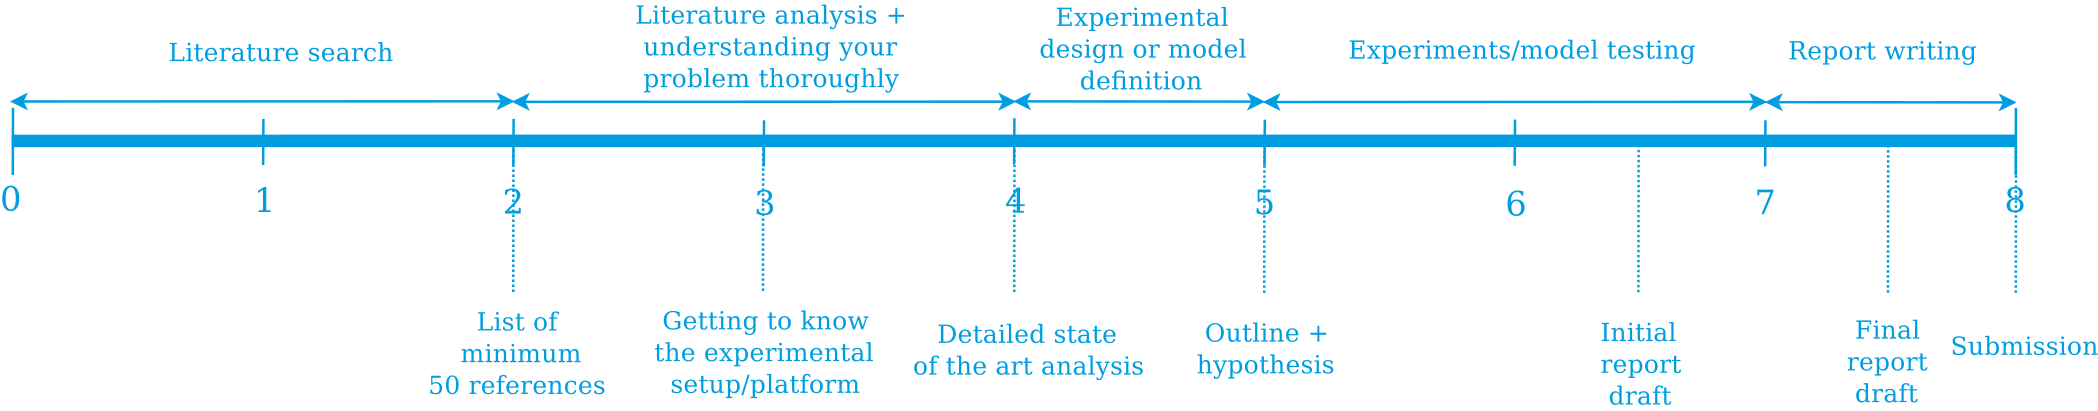
\includegraphics[width=\textwidth]{images/rnd_deliverable_timeline}
    \caption{My figure caption}
    \label{fig:myfigure}
\end{figure}

\subsection{Deliverables}

\subsubsection*{Minimum Viable}
\begin{itemize}
    \item This project aims to create a framework for real-time learning from demonstration and lifetime learning based on a graph representation of the environment, with the possibility of mapping obstacles and objects. The experiments will be performed by QTrobot and tested with real non-expert demonstrators. 
\end{itemize}
\subsubsection*{Expected}
\begin{itemize}
    \item The framework can be generalised and extended to the use of NAO and Kinova arms, aka Freddy robot, due to the higher amount of DOF, to prove that the framework can be extended to any robot with two arms. 
\end{itemize}
\subsubsection*{Desired}
\begin{itemize}
    \item As the focus of this project is on a friendly system, it is desirable, but not necessary, to have at the top of the framework an interactive set of voice commands to start and stop the recordings, as well as to stop in case of emergency, this for the robots with integrated microphones.
\end{itemize}

\nocite{*}

\bibliographystyle{plainnat} % Use the plainnat bibliography style
\bibliography{bibliography.bib} % Use the bibliography.bib file as the source of references

\end{document}
